%%%%%%%%%%%%%%%%%%%%%%%%%%%%%%%%%%%%%%%%%%%%%%%%%%%%%%%
%                File: OpEx_style.tex                 %
%                  Date: Sept. 2, 2009                %
%                                                     %
%           LaTeX template file for use with          %
%           OSA's journal Optics Express              %
%                                                     %
%  send comments to Jennifer Mayfield, jmayfi@osa.org %
%                                                     %
% This file requires style file, opex3.sty, under     %
%              the LaTeX article class                %
%                                                     %
%   \documentclass[10pt,letterpaper]{article}         %
%   \usepackage{opex3}                                %
%                                                     %
% Note that our online submission system does not     %
% currently process PDFLaTeX; if PDFLaTeX must be     %
% used, pls. contact OpEx staff, and we will process  %
% manually                                            %
%                                                     %
%                                                     %
%       (c) 2009 Optical Society of America           %
%%%%%%%%%%%%%%%%%%%%%%%%%%%%%%%%%%%%%%%%%%%%%%%%%%%%%%%

%%%%%%%%%%%%%%%%%%%%%%% preamble %%%%%%%%%%%%%%%%%%%%%%%%%%%
\documentclass[10pt,letterpaper]{article}
\usepackage{opex3}


%%%%%%%%%%%%%%%%%%%%%%% begin %%%%%%%%%%%%%%%%%%%%%%%%%%%%%%
\begin{document}

%% NOTE: TITLE PAGE & TOC NOT USED FOR MANUSCRIPT SUBMISSIONS %%
\title{Template and style guide for authors submitting to \textit{Optics Express}}

\vskip4pc

\tableofcontents
\clearpage
%% NO TITLE PAGE FOR OPEX SUBMISSIONS %%

%% START HERE
%%%%%%%%%%%%%%%%%% title page information %%%%%%%%%%%%%%%%%%
\title{Template and style guide for authors submitting to \textit{Optics Express}}

\author{M. Scott Dineen and Jennifer Mayfield}

\address{Optics Express Office, Publications Department, Optical Society of America, \\ Washington, D.C., 20036}

\email{opex@osa.org} %% email address is required

% \homepage{http:...} %% author's URL, if desired

%%%%%%%%%%%%%%%%%%% abstract and OCIS codes %%%%%%%%%%%%%%%%
%% [use \begin{abstract*}...\end{abstract*} if exempt from copyright]

\begin{abstract} A template and instructions are provided for preparing \textit{Optics Express} manuscripts in \LaTeX. A basic template, \texttt{OpEx\_temp.tex}, is also provided. Note that the style file \texttt{opex3.sty} replaces \texttt{opex2.sty}. Additional information on style and submissions is available at \mbox{\url{http://www.opticsexpress.org/submission}}.\end{abstract}

\ocis{(000.0000) General.} % REPLACE WITH CORRECT OCIS CODES FOR YOUR ARTICLE

%%%%%%%%%%%%%%%%%%%%%%% References %%%%%%%%%%%%%%%%%%%%%%%%%
\begin{thebibliography}{99}
\bibitem{gallo99} K. Gallo and G. Assanto, ``All-optical diode based on second-harmonic generation in an asymmetric waveguide,'' \josab {\bf 16,} 267--269 (1999).
 
\bibitem{Masters98a} B. R. Masters, ``Three-dimensional microscopic tomographic imagings of the cataract in a human lens in vivo,'' \opex {\bf 3,} 332--338 (1998), \url{http://www.opticsexpress.org/abstract.cfm?URI=OPEX-3-9-332}.
 
\bibitem{Oron03} D. Yelin,  D. Oron,  S. Thiberge,  E. Moses, and Y. Silberberg, ``Multiphoton plasmon-resonance microscopy,'' \opex {\bf 11,} 1385--1391 (2003), \url{http://www.opticsexpress.org/abstract.cfm?URI=OPEX-11-12-1385}.
\end{thebibliography}

%%%%%%%%%%%%%%%%%%%%%%%%%%  body  %%%%%%%%%%%%%%%%%%%%%%%%%%
\section{Introduction}
Adherence to the specifications listed in this template is essential for efficient review and publication of submissions. Since OSA does not routinely perform copyediting and typesetting for this journal, use of the template is critical to providing a consistent appearance. Proper reference format is especially important (see Section \ref{sec:refs}).

\section{\texttt{opex3.sty} and required \LaTeX{} packages}
Page layout is set with the \texttt{geometry} package for US Letter paper. \texttt{opex3.sty} uses the following package files:

\begin{itemize}
\item \texttt{geometry} \ (page layout)
\item \texttt{color, graphicx} \ (replaces \texttt{graphics}; has preset options)
\item \texttt{mathptmx, courier, helvet} \ (Times, Courier, and Helvetica fonts) 
\end{itemize}

The latest versions of these standard package files can be obtained at CTAN: the Comprehensive TeX Archive Network, \url{http://www.ctan.org}.

\bigskip

\noindent The command \verb+\usepackage{ae}+ can be invoked to revert font to Computer Modern, although we prefer to publish with Times (with \texttt{mathptmx.sty}) for consistency.

\begin{figure}[htb]
\centering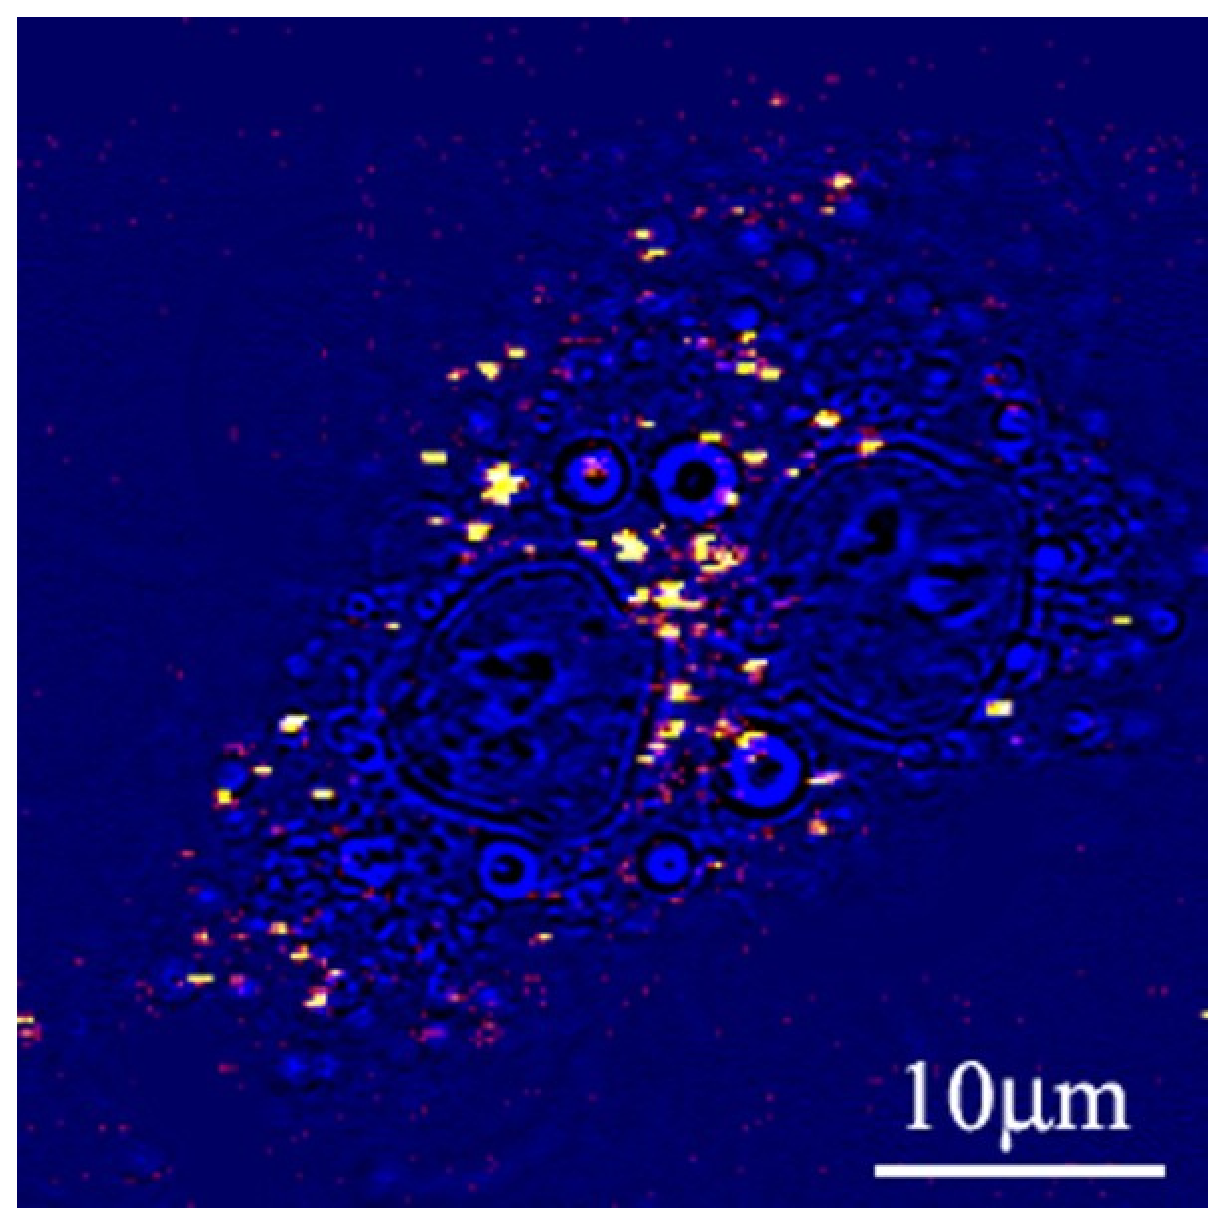
\includegraphics[width=7cm]{opexfig1}
\caption{Sample caption (Ref. \cite{Oron03}, Fig. 2).}
\end{figure}

\section{Figures, tables, and multimedia}
\textit{Optics Express} encourages authors to submit color and multimedia figures with their manuscripts. Guidelines on multimedia submissions can be found at \mbox{\url{http://www.opticsexpress.org/submission/multimedia.cfm}}. Figures and tables should be placed in the body of the manuscript. To include multimedia, set a static image (e.g., frame from a video) in the manuscript as a figure, and upload multimedia files separately.

\bigskip

\noindent Standard \LaTeX{} environments should be used to place tables and figures:
\begin{verbatim}
\begin{figure}[htbp]
\centering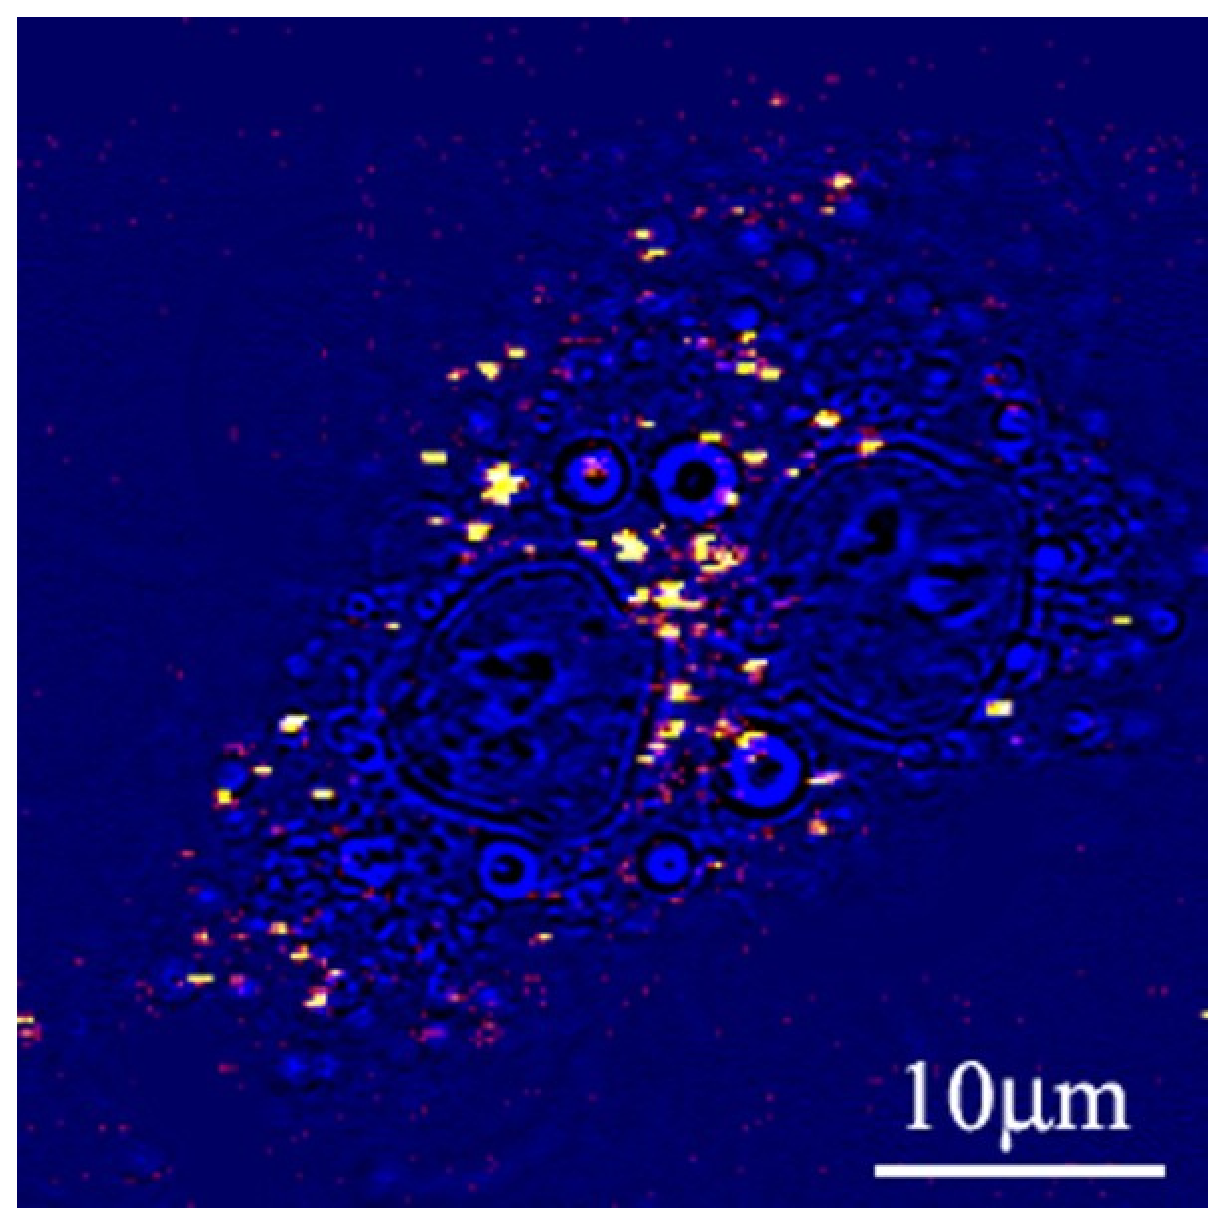
\includegraphics[width=7cm]{opexfig1}
\caption{Sample caption (Ref. \cite{Oron03}, Fig. 2).}
\end{figure}
\end{verbatim}
\section{Mathematical and scientific notation}
\subsection{Displayed equations} Displayed equations should be centered.
Equation numbers should appear at the right-hand margin, in
parentheses:
\begin{equation}
H = \frac{1}{2m}(p_x^2 + p_y^2) + \frac{1}{2} M{\Omega}^2
     (x^2 + y^2) + \omega (x p_y - y p_x).
\end{equation}

All equations should be numbered in the order in which they appear
and should be referenced  from within the main text as Eq. (1),
Eq. (2), and so on [or as inequality (1), etc., as appropriate].

\subsection{Inline math} To help with conversion, place all math in a proper math environment. For example, expression \mbox{$3\times 4 = 12$} should be set this way, \texttt{\$3$\backslash$times 4=12\$}, not this way, \texttt{3 \$$\backslash$times\$4=12}. Simple fractions for inline math
should use parentheses when necessary to avoid ambiguity, for
example, to distinguish between $1/(n-1)$ and $1/n-1$.  Exceptions
to this are the proper fractions such as $\frac{1}{2}$, which are
better left in this form. Summations and integrals that appear
within text such as $\frac{1}{2}{\sum }_{n=1}^{n=\infty} (n^2 -
2n)^{-1}$ should have limits placed to the right of the symbol to
reduce white space.

\subsection{General guidelines on notation} Notation must be
legible, clear, compact, and consistent with standard usage. In
general, acronyms should be defined at first use. Adherence to the
following guidelines will greatly assist the production process:

\paragraph*{\bf Radical signs.}
When possible, avoid oversized radical signs
by using the notation of a superscript $1/2$. For example, change
$\sqrt{(a + b)(a - c)}$ to $[(a + b)(a - c)]^{1/2}$.

\paragraph*{\bf Exponentials.} Avoid tiny superscripts of exponential $e$ (e.g.,
$e^{jkl})$ by using the alternative \verb+\exp+ notation,
$\exp(jkl)$.

\paragraph*{\bf Variables and vectors.}
Set single-letter variables in italics $(k)$. Set three-vectors in
boldface $(\mathbf{k})$. Functions, derivative ``d,''
abbreviations, and multiletter identifiers should be set in roman
(plain) type  ($\alpha \cos, \int\!\dots{\rm d}x, k^{\rm out}$).

\paragraph*{\bf Multiplication.}
In general, close up multiplied terms $(p_yp_x)$;
use $\times$ if multiplication sign is essential $(2 \times
10^{-2})$ or for continuation in displayed equations. Use raised dot only for scalar product $(\mathbf{k \cdot k})$.

\paragraph*{\bf Fences.}
For simple bracketing the usual order of parentheses and brackets
is $\{ \, [  \, (  \,  \{  \, [  \, (  \, |  \, )  \, ]  \, \} \,
)  \, ]  \, \}$.


\paragraph*{\bf Metric system.}
The metric system is used in OSA journals. If nonmetric units are
essential (e.g., for parts specifications), conversion should be
given at first mention:  ``. . . a $\frac{1}{4}$\,-in. bolt \mbox{(1 in.
= 2.54 cm).''}

\subsection{Acknowledgments} Acknowledgments, if included, should
appear at the end of the document, just before the references. The
number of a grant or contract should be omitted unless its
inclusion is required by the agency supporting the research. Use
the command \verb+\section*{Acknowledgments}+  to create a
nonnumbered section heading.
\section{References}
\label{sec:refs}
Proper formatting of references is extremely important, not only for consistent appearance but also for accurate electronic tagging. Please follow the guidelines provided below on formatting, callouts, and use of Bib\TeX.

\subsection{Formatting reference items}
Each source must have its own reference number. Footnotes (notes
at the bottom of text pages) are not used in OSA journals.
References require all author names, full titles, and inclusive
pagination. Here are some examples of how to set the most common
reference types:

\bigskip

\hskip8pt{\bf Journal paper}

\begin {enumerate}

\item C. van Trigt, ``Visual system-response functions and estimating reflectance,'' %\josaa
   J. Opt. Soc. Am. A {\bf 14,} 741--755 (1997).

\vskip.4pc  {\bf Book}

\item T. Masters, {\it Practical Neural Network Recipes in C++} (Academic,
New York, 1993).

\vskip.4pc {\bf Chapter in a book}

\item B. L. Shoop, A. H. Sayles, and D. M. Litynski, ``New devices for
optoelectronics:  \ smart pixels,'' in {\it Handbook of Fiber
Optic Data Communications,} C. DeCusatis, D. Clement, E. Maass,
and R. Lasky, eds. (Academic, San Diego, Calif., 1997), pp.
705--758.

\vskip.4pc {\bf Paper in a published conference proceedings}

\item R. E. Kalman, ``Algebraic aspects of the generalized inverse of a
rectangular matrix,'' in {\it Proceedings of Advanced Seminar on
Genralized Inverse and Applications,} M. Z. Nashed, ed. (Academic,
San Diego, Calif., 1976), pp. 111--124.

\vskip.4pc {\bf Paper in an unpublished conference proceedings}

\item D. Steup and J. Weinzierl, ``Resonant THz-meshes,'' presented at the
Fourth International Workshop on THz Electronics,
Erlangen-Tennenlohe, Germany, 5--6 Sept. 1996.

\vskip.4pc {\bf SPIE proceedings}

\item S. K. Griebel, M. Richardson, K. E. Devenport, and H. S. Hinton,
``Experimental performance of an ATM-based buffered hyperplane
CMOS-SEED smart pixel array,'' in {\it Optoelectronic
Interconnects and Packaging IV,} R. T. Chen and P. S. Guilfoyle,
eds., Proc. SPIE {\bf 3005,} 254--256 (1997).

\vskip.4pc {\bf IEEE proceedings}

\item T. Darrel and K. Wohn, ``Pyramid based depth from focus,'' in
{\it Proceedings of IEEE Conference on Computer Vision and Pattern
Recognition} (Institute of Electrical and Electronics Engineers,
New York, 1988), pp. 504--509.

\vskip.4pc {\bf OSA proceedings}

\item W. J. Alford, T. D. Raymond, and A. V. Smith, ``Characterization of a ring optical
parametric oscillator,'' in {\it Advanced Solid-State Lasers,} T.~
Y. Fan and B. Chai, eds., Vol. 20 of OSA Proceedings Series
(Optical Society of America, Washington, D.C., 1994), pp.
476--479.

\vskip.4pc {\bf Personal communication}

\item Barbara Williams, Editorial Department, Optical Society of
America, 2010 Massa\-chusetts Avenue, N.W., Washington, D.C.,
20036 (personal communication, 2001).

\vskip.4pc{\bf Electronic archives and Internet sources}

{\em Electronic periodical}

\item C. Jerry, ``Remarks on the use of group
theory in quantum optics,'' \opex {\bf 8,} 76--85 (2001),
\url{http://www.opticsexpress.org/abstract.cfm?URI=OPEX-8-2-76}.

\end{enumerate}
The commands \verb+\begin{thebibliography}{}+ and
\verb+\end{thebibliography}+ format the section according to
standard style, showing the title {\bf References and links}.  Use the
\verb+\bibitem{label}+ command to start each reference.
\subsection{Formatting reference citations}
References should be numbered consecutively in the order in which
they are referenced in the body of the paper. Set reference callouts with standard \verb+\cite{}+ command or set manually inside square brackets [1]. 

\subsection{Bib\TeX}
\label{sec:bibtex}
Bib\TeX{} may be used to create a file containing the references, whose contents (i.e., contents of \texttt{.bbl} file) can then be pasted into the bibliography section of the \texttt{.tex} file. A new Bib\TeX{} style file, \texttt{osajnl.bst}, is provided.

To assist authors with journal abbreviations in references, standard abbreviations for 31 commonly cited journals have been included as macros within opex3.sty.  The abbreviations are shown in Table 1. 

\begin{table}[htb]
\centering\caption{Standard abbreviations
 for 31 commonly cited journals.}
\begin{tabular}{lp{1.7in}|lp{1.7in}}
\hline 
Macro & Abbreviation & Macro & Abbreviation \\ \hline
\verb+\ao+ & Appl.\  Opt.\     \\
\verb+\ap+ & Appl.\  Phys.\  & \verb+\nat+ & Nature (London)   \\
\verb+\apl+ & Appl.\ Phys.\ Lett.\
  & \verb+\oc+ & Opt.\ Commun.\  \\
\verb+\apj+ & Astrophys.\ J.\  & \verb+\opex+ & Opt.\ Express    \\
\verb+\bell+ & Bell Syst.\ Tech.\ J.\
  & \verb+\ol+ & Opt.\ Lett.\   \\
\verb+\jqe+ & IEEE J.\ Quantum Electron.\
  & \verb+\pl+ & Phys.\ Lett.\   \\
\verb+\assp+ & IEEE Trans.\ Acoust.\ Speech Signal Process.\
  & \verb+\pra+ & Phys.\ Rev.\ A   \\
\verb+\aprop+ & IEEE Trans.\  Antennas Propag.\ 
  & \verb+\prb+ & Phys.\ Rev.\ B   \\
\verb+\mtt+ & IEEE Trans.\ Microwave Theory Tech.\
  & \verb+\prc+ & Phys.\ Rev.\ C   \\
\verb+\iovs+ & Invest.\ Ophthalmol.\ Vis.\ Sci.\
  & \verb+\prd+ & Phys.\ Rev.\ D   \\
\verb+\jcp+ & J.\ Chem.\ Phys.\
  & \verb+\pre+ & Phys.\ Rev.\ E   \\
\verb+\jmo+ & J.\ Mod.\ Opt.\
  & \verb+\prl+ & Phys.\ Rev.\ Lett.\    \\
\verb+\jon+ & J.\ Opt.\ Netw.\ 
  & \verb+\rmp+ & Rev.\ Mod.\ Phys.\    \\
\verb+\josa+ & J.\ Opt.\ Soc.\ Am.\  
  & \verb+\pspie+ & Proc.\ Soc.\ Photo-Opt.\ Instrum.\ Eng.\   \\
\verb+\josaa+ & J.\ Opt.\ Soc.\ Am.\ A 
  & \verb+\sjqe+ & Sov.\ J.\ Quantum Electron.\   \\
\verb+\josab+ & J.\ Opt.\ Soc.\ Am.\ B
  & \verb+\vr+ & Vision Res.\   \\
\verb+\jpp+ & J.\ Phys.\ (Paris)  & &  \\ \hline
\end{tabular}
\end{table}

\section{Conclusion}
After proofreading the manuscript, tar and gzip the \texttt{.tex} file and
figures; then enter the requested information into the \textit{Optics Express}
online submission system at \url{http://www.opticsexpress.org} and upload the tarred and gzipped archive. If there is video or other multimedia, the associated files should be uploaded separately.

\end{document}
